%------------------------------------------------------------------------------
% 
% by Quentin Bammey, Marina Gardella, Tina Nikoukhah, Miguel Colom, Jean-Michel Morel, Rafael Grompone von Gioi
%------------------------------------------------------------------------------
\documentclass{ipol}

\ipolSetTitle{Image Forgeries detection through Mosaic Analysis: the Intermediate Values Algorithm}
\ipolSetAuthors{Quentin Bammey, Rafael Grompone von Gioi, Jean-Michel Morel}

\ipolSetAffiliations{Universit\'e Paris-Saclay, ENS Paris-Saclay, CNRS, Centre Borelli, F-94235, Cachan, France \\
\texttt{\{quentin.bammey, rafael.grompone, jean-michel.morel\}@ens-paris-saclay.fr}}

%------------------------------------------------------------------------------
\ipolPreprintLink{http://www.ipol.im/}

%------------------------------------------------------------------------------
\usepackage{subcaption}
\usepackage[dvipsnames]{xcolor}

%All the colours we used for the database articles. c0, c1, c2 and c3 go nicely together
\definecolor{c0}{HTML}{0E918C}
\definecolor{c1}{HTML}{F6830F}
\definecolor{c2}{HTML}{BB2205}
\definecolor{c3}{HTML}{1F3C88}
\definecolor{grayA}{HTML}{D2D3C9}
\definecolor{cgray}{HTML}{708090}
\definecolor{cgreen}{HTML}{1F8C88}
\usepackage[vlined,algoruled,linesnumbered]{algorithm2e}
\usepackage{namedinput}

\SetKwNamedIO{Input}{Input}
\SetKwNamedIO{Parameter}{Param}
\SetKwNamedIO{Output}{Output}
%\SetKwInOut{dontusethis}{aaaaaaaaaaaaaa}  % hack to get enough spacing for names
\renewcommand{\KwSty}[1]{\textnormal{\textcolor{c1}{\ttfamily\bfseries #1}}\unskip}
\renewcommand{\ArgSty}[1]{\textnormal{\ttfamily #1}\unskip}
\renewcommand{\DataSty}[1]{\color{c2}\bfseries #1}
\SetKwComment{Comment}{\color{c0}\# }{}
\renewcommand{\CommentSty}[1]{\textnormal{\ttfamily\color{c0}#1}\unskip}
\newcommand{\assign}{:\!=}
\newcommand{\peq}{+\mkern-8mu=}
\newcommand{\var}{\texttt}
\newcommand{\FuncCall}[2]{\texttt{\bfseries #1(#2)}}
\SetKwProg{Function}{function}{}{}
\renewcommand{\ProgSty}[1]{\texttt{\bfseries \color{c3}#1}}
\DontPrintSemicolon
\SetKw{IN}{in}
\SetKw{AND}{and}
\SetKw{FROM}{from}
\SetKw{TO}{to}
%\newcommand{\IN}{~\KwSty{in}~}
%\newcommand{\FROM}{~\KwSty{from}~}
%\newcommand{\TO}{~\KwSty{to}~}
\usepackage{booktabs} % table

\usepackage{amsmath, amssymb}
\DeclareMathOperator*{\argmax}{arg\,max}

%------------------------------------------------------------------------------
\begin{document}


\begin{ipolAbstract}
Here is the abstract.
\end{ipolAbstract}

\begin{ipolCode}
The reviewed source code and documentation for this algorithm are
available from \href{\ipolLink}{the web page of this
article}. Usage instruction are included in the
\verb|README.txt| file of the archive.
\end{ipolCode}

\begin{ipolSupp}
The link to the demo is \href{}{}.
\end{ipolSupp}

\ipolKeywords{image forensics, forgery detection}
\newpage

%------------------------------------------------------------------------------
\section{Introduction}

%------------------------------------------------------------------------------
\section{Method}

%------------------------------------------------------------------------------
\section{Algorithm}

\begin{algorithm}[h]
\caption{Mark intermediate values (original isotropic version)}
\label{alg:intermediate}
\Function{is\_intermediate(arr)}{
\Input{arr}{Array of size $(X, Y)$, one channel of an image}
\Output{mask}{Array of size $(X-4, Y-4)$, intermediate values mask}

mask $\assign \mathbf 0_{(X-4, Y-4)}$\;
\For{$x$ \FROM 2 \TO $X-2$ \AND $y$ \FROM 2 \TO $Y-2$}{
$\mathrm{mi}\assign \min{(\mathrm{arr}_{x+1, y}, \mathrm{arr}_{x, y-1}, \mathrm{arr}_{x-1, y}, \mathrm{arr}_{x, y+1})}$\;
$\mathrm{ma}\assign \max{(\mathrm{arr}_{x+1, y}, \mathrm{arr}_{x, y-1}, \mathrm{arr}_{x-1, y}, \mathrm{arr}_{x, y+1})}$\;
\If{$\mathrm{mi} \leq \mathrm{arr}_{x, y} \leq \mathrm{ma}$}
{
    $\mathrm{mask}_{x-2, y-2}\assign 1$\;
}
}
\Return{mask}
}
\end{algorithm}

\begin{algorithm}[h]
\caption{Mark intermediate values (bidirectional variant)}
\label{alg:intermediate_bidirectional}
\Function{is\_intermediate(arr)}{
\Input{arr}{Array of size $(X, Y)$, one channel of an image}
\Output{mask}{Array of size $(X-4, Y-4)$, intermediate values mask}

mask $\assign \mathbf 0_{(X-4, Y-4)}$\;
\For{$x$ \FROM 2 \TO $X-2$ \AND $y$ \FROM 2 \TO $Y-2$}{
$\mathrm{mi}_h\assign \min(\mathrm{arr}_{x-1, y}, \mathrm{arr}_{x+1, y}$\;
$\mathrm{ma}_h\assign \max(\mathrm{arr}_{x-1, y}, \mathrm{arr}_{x+1, y}$\;
$\mathrm{mi}_v\assign \min(\mathrm{arr}_{x, y-1}, \mathrm{arr}_{x, y+1}$\;
$\mathrm{ma}_v\assign \max(\mathrm{arr}_{x, y-1}, \mathrm{arr}_{x, y+1}$\;

\If{$\mathrm{mi_h} \leq \mathrm{arr}_{x, y} \leq \mathrm{ma_h}$}
{
    $\mathrm{mask}_{x-2, y-2}\peq \frac 1 2$\;
}
\If{$\mathrm{mi_v} \leq \mathrm{arr}_{x, y} \leq \mathrm{ma_v}$}
{
    $\mathrm{mask}_{x-2, y-2}\peq \frac 1 2$\;
}
}
\Return{mask}
}
\end{algorithm}

\begin{algorithm}[h]
\caption{Find the grid}
\label{alg:grid}
\Function{find\_grid($R, G, B$)}
{
\Input{$R$}{Array of size $(X, Y)$, typically as returned by \FuncSty{is\_intermediate} or a sub-window of it on the red channel}
\Input{$G$}{Same as above for the green channel}
\Input{$B$}{Same as above for the blue channel}
\Output{main}{CFA pattern identified by the function (one of \textsc{rggb}, \textsc{grbg}, \textsc{gbrg}, \textsc{bggr})}
\Output{diag}{Diagonal pattern identified by the function (either \textsc{·gg·} or \textsc{g··g})}
\Output{diff\_main}{Difference of count in intermediate values between the two pattern sharing the same diagonal. Positive if the best pattern is \textsc{rggb} or \textsc{grbg}, negative if the best pattern is \textsc{gbrg} or \textsc{bggr}.}
\Output{diff\_diag}{Difference of count of intermediate values between the two diagonal patterns.}
\Comment{First we select the best diagonal pattern using the green values}
$\mathrm{count_{*GG*}}\assign \sum_{x=0}^{\frac X 2}G_{2x,2y+1} + G_{2x+1, 2y}$\;
$\mathrm{count_{G**G}}\assign \sum_{x=0}^{\frac X 2}G_{2x,2y} + G_{2x+1, 2y+1}$\;
$\mathrm{diff\_diag} \assign \frac 2{XY}\left(\mathrm{count_{*GG*}} - \mathrm{count_{G**G}}\right)$\;
\If{$\mathrm{diff\_diag}$ < 0}{
main$\assign$ \textsc{·gg·}\;
}
\Else{
main$\assign$ \textsc{g··g}\;
}

\Comment{Now we select within the two patterns sharing the detected diagonal.}
\If{diff\_diag$=$\textsc{·gg·}}
{
\Comment{Either \textsc{rggb} or \textsc{bggr}}
$\mathrm{count_{RGGB}}\assign \sum_{x=0}^{\frac X 2}R_{2x,2y} + B_{2x+1, 2y+1}$\;
$\mathrm{count_{BGGR}}\assign \sum_{x=0}^{\frac X 2}R_{2x+1,2y+1} + B_{2x, 2y}$\;
$\mathrm{diff\_main} \assign \frac 2{XY}\left(\mathrm{count_{RGGB}} - \mathrm{count_{BGGR}}\right)$\;
\If{$\mathrm{diff\_main}$ < 0}{
main$\assign$ \textsc{rggb}\;
}
\Else{
main$\assign$ \textsc{bggr}\;
}
}
\Else
{
\Comment{Either \textsc{grbg} or \textsc{gbrg}}
$\mathrm{count_{GRBG}}\assign \sum_{x=0}^{\frac X 2}R_{2x+1,2y} + B_{2x, 2y+1}$\;
$\mathrm{count_{GBRG}}\assign \sum_{x=0}^{\frac X 2}R_{2x,2y+1} + B_{2x+1, 2y}$\;
$\mathrm{diff\_main} \assign \frac 2{XY}\left(\mathrm{count_{GRBG}} - \mathrm{count_{GBRG}}\right)$\;
\If{$\mathrm{diff\_main}$ < 0}{
main$\assign$ \textsc{grbg}\;
}
\Else{
main$\assign$ \textsc{gbrg}\;
}
}
\Return{main, diag, diff\_main, diff\_diag}
}
\end{algorithm}


\clearpage




%------------------------------------------------------------------------------
\section{Experiments}
To evaluate the ability of this method to detect the CFA pattern correctly, we take 15 images from the Raise Dataset~\cite{raise}, and demosaick them using the 7 algorithms available in LibRaw: Bilinear interpolation, AAHD, AHD, DCB, DHT, PPG and VNG. 11 of these images are of size $4948\times3280$, the other 4 are of size $4310\times2868$. The selected images can be seen in Fig.~\ref{fig:15images}.

\begin{figure}[ht]
    \centering
    \begin{subfigure}[c]{.31\linewidth}\centering
    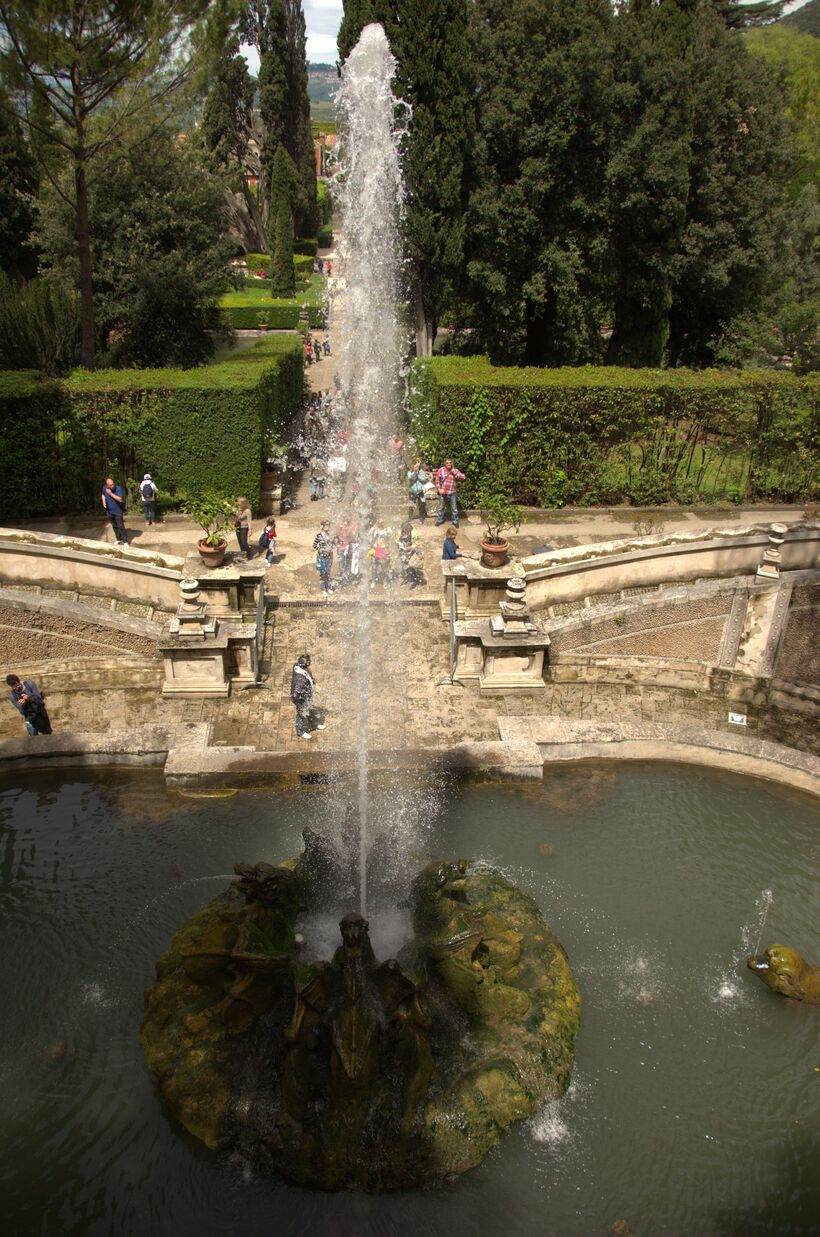
\includegraphics[height=\linewidth]{images/original/r002fc3e2t.jpeg}
    \caption{r002fc3e2t}
    \end{subfigure}\hfill%
    \begin{subfigure}[c]{.31\linewidth}\centering
    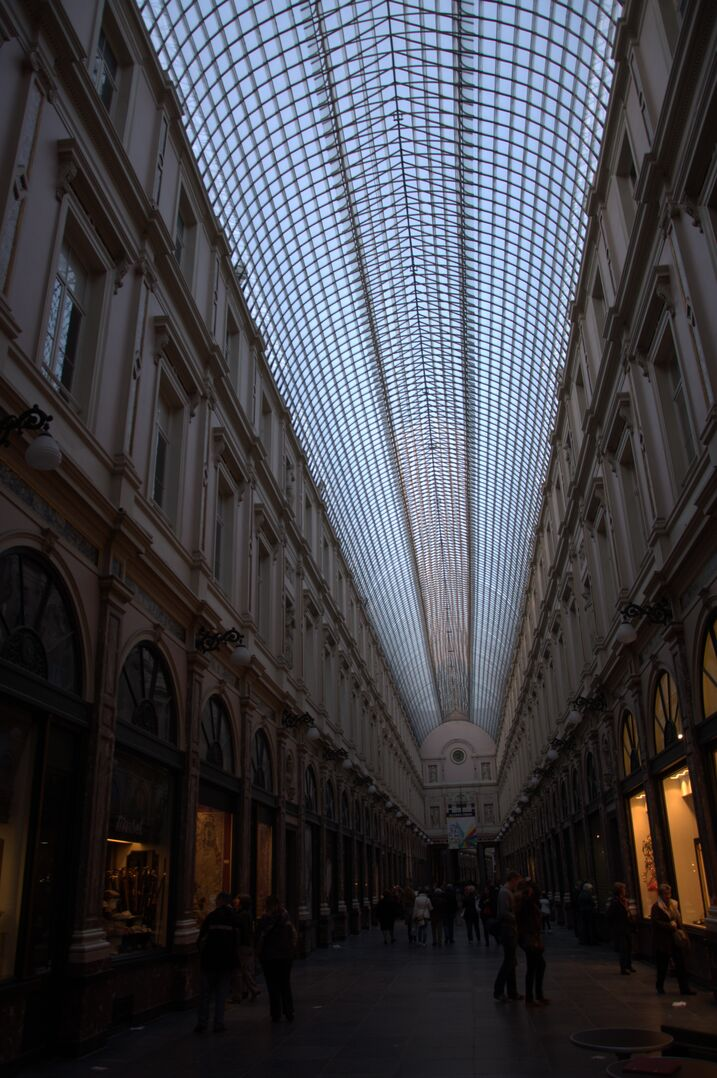
\includegraphics[height=\linewidth]{images/original/r1ead3024t.jpeg}
    \caption{r1ead3024t}
    \end{subfigure}\hfill%
    \begin{subfigure}[c]{.31\linewidth}\centering
    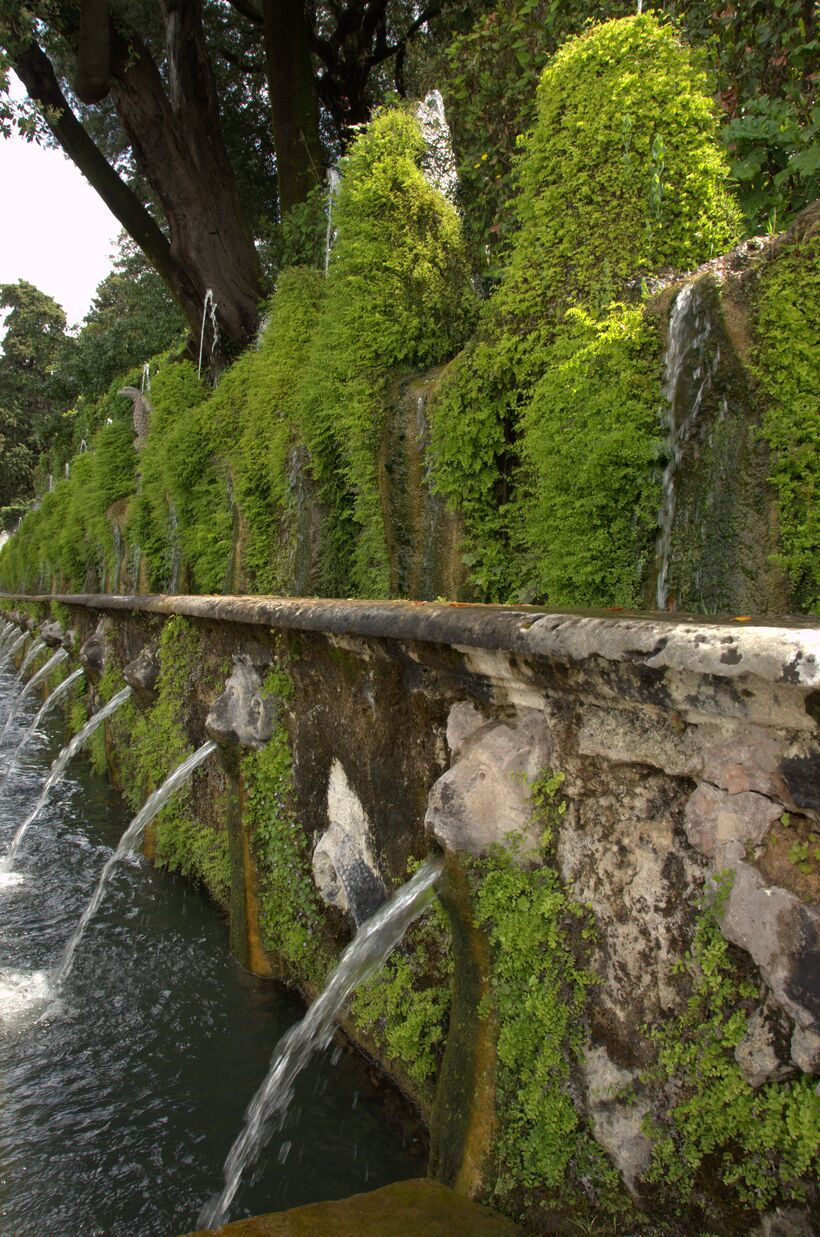
\includegraphics[height=\linewidth]{images/original/r1ceba29dt.jpeg}
    \caption{r1ceba29dt}
    \end{subfigure}%
    
    \begin{subfigure}[c]{.31\linewidth}\centering
    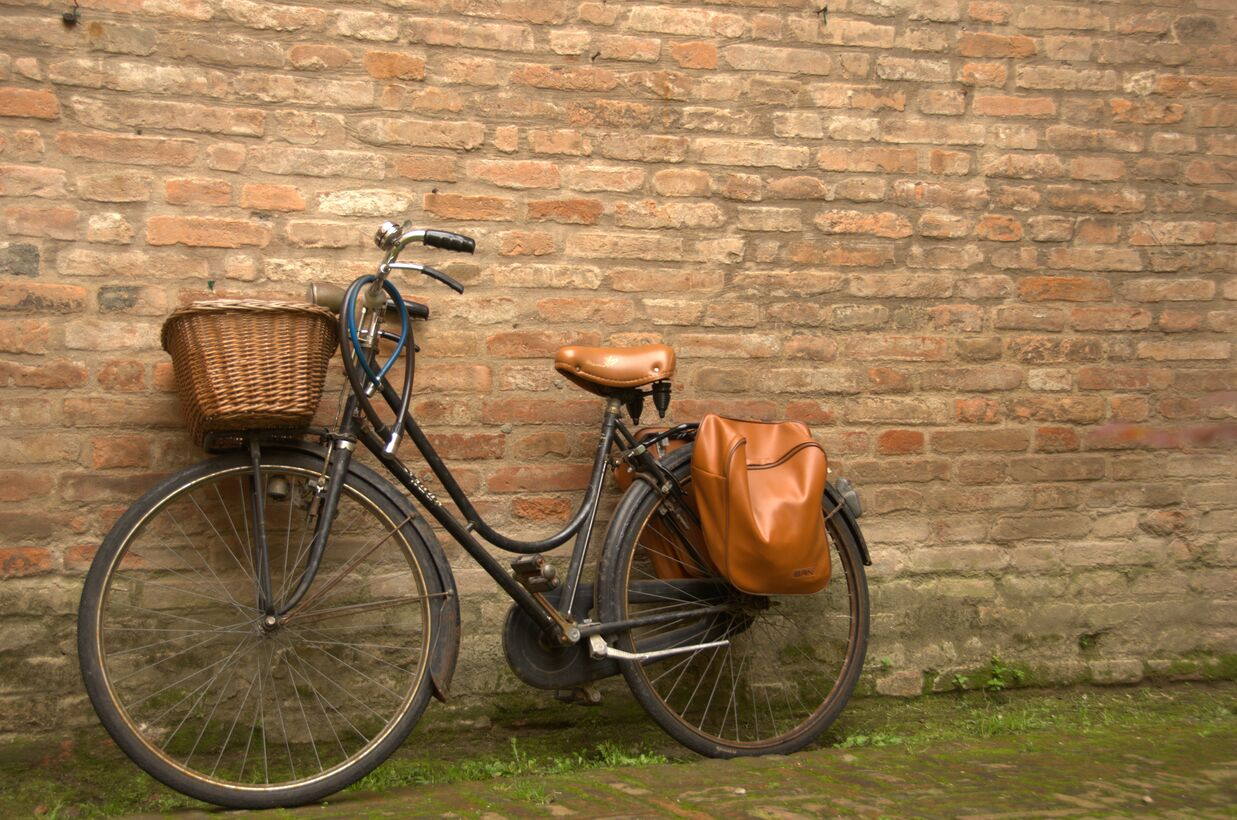
\includegraphics[width=\linewidth]{images/original/r0a2ff882t.jpeg}
    \caption{r0a2ff882t}
    \end{subfigure}\hfill%
    \begin{subfigure}[c]{.31\linewidth}\centering
    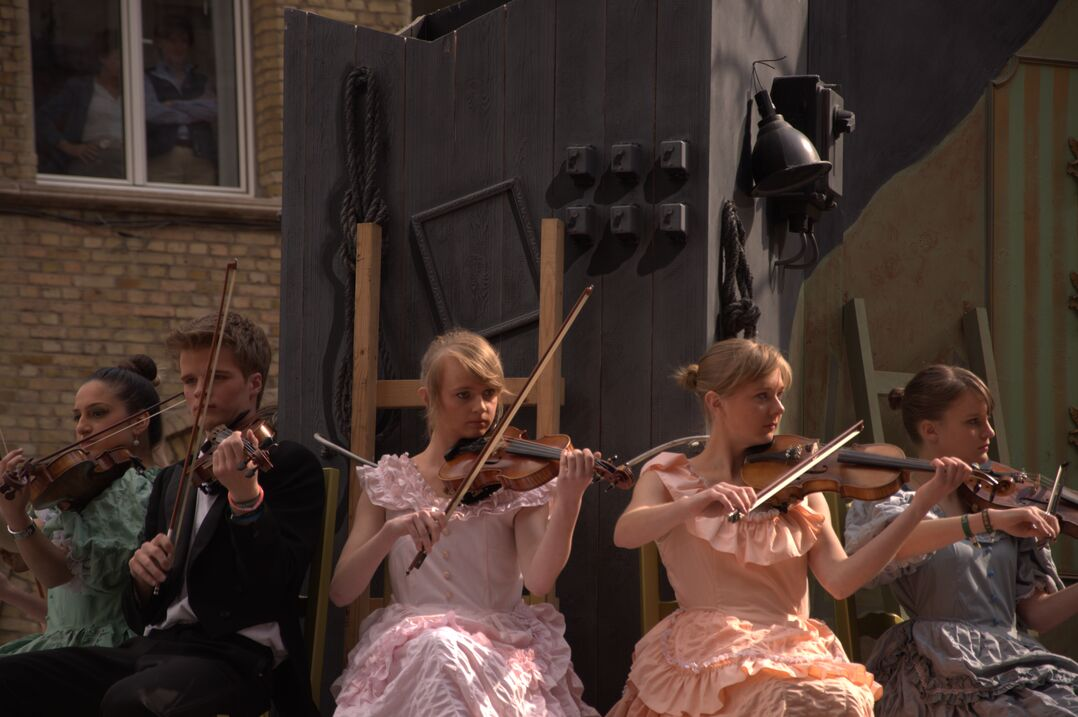
\includegraphics[width=\linewidth]{images/original/r0a808003t.jpeg}
    \caption{r0a966704t}
    \end{subfigure}\hfill%
    \begin{subfigure}[c]{.31\linewidth}\centering
    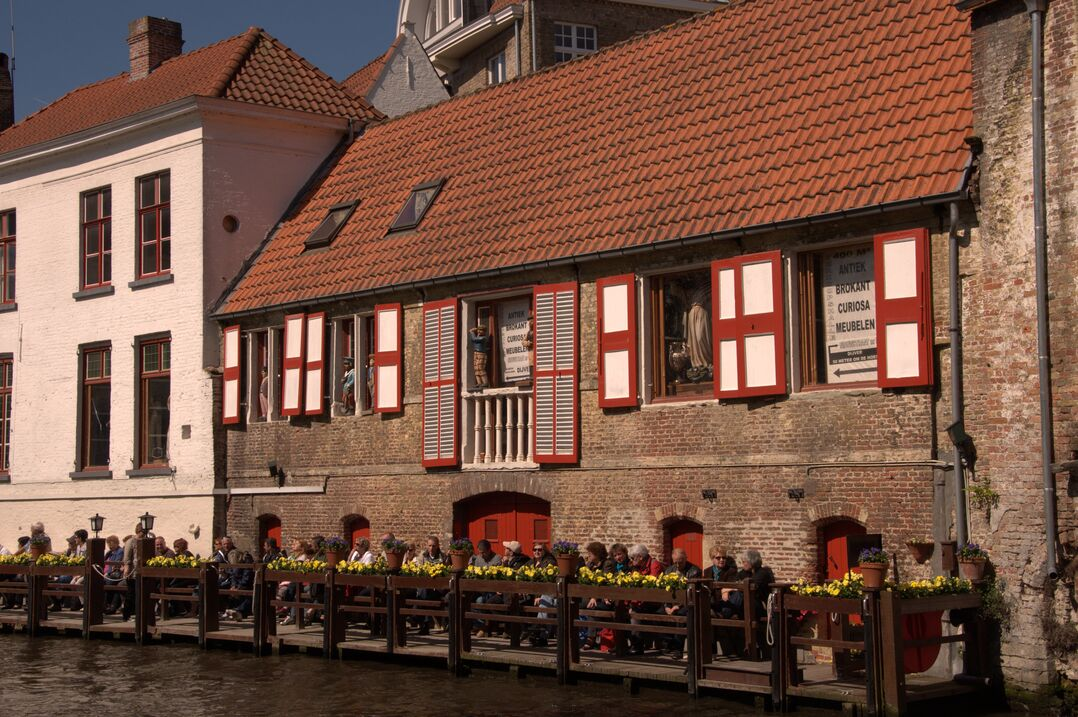
\includegraphics[width=\linewidth]{images/original/r0a966704t.jpeg}
    \caption{r0ea0825ft}
    \end{subfigure}
    
    \begin{subfigure}[c]{.31\linewidth}\centering
    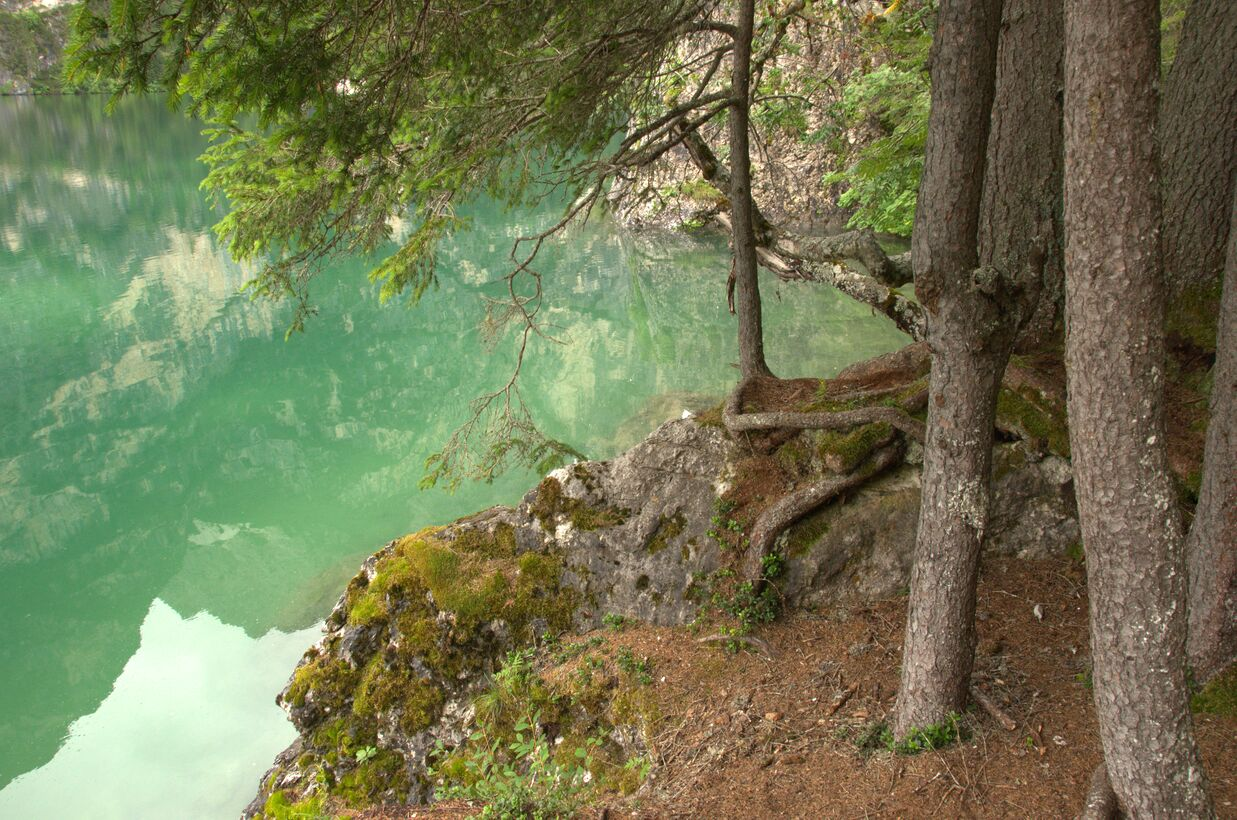
\includegraphics[width=\linewidth]{images/original/r0e04cc91t.jpeg}
    \caption{r0a2ff882t}
    \end{subfigure}\hfill%
    \begin{subfigure}[c]{.31\linewidth}\centering
    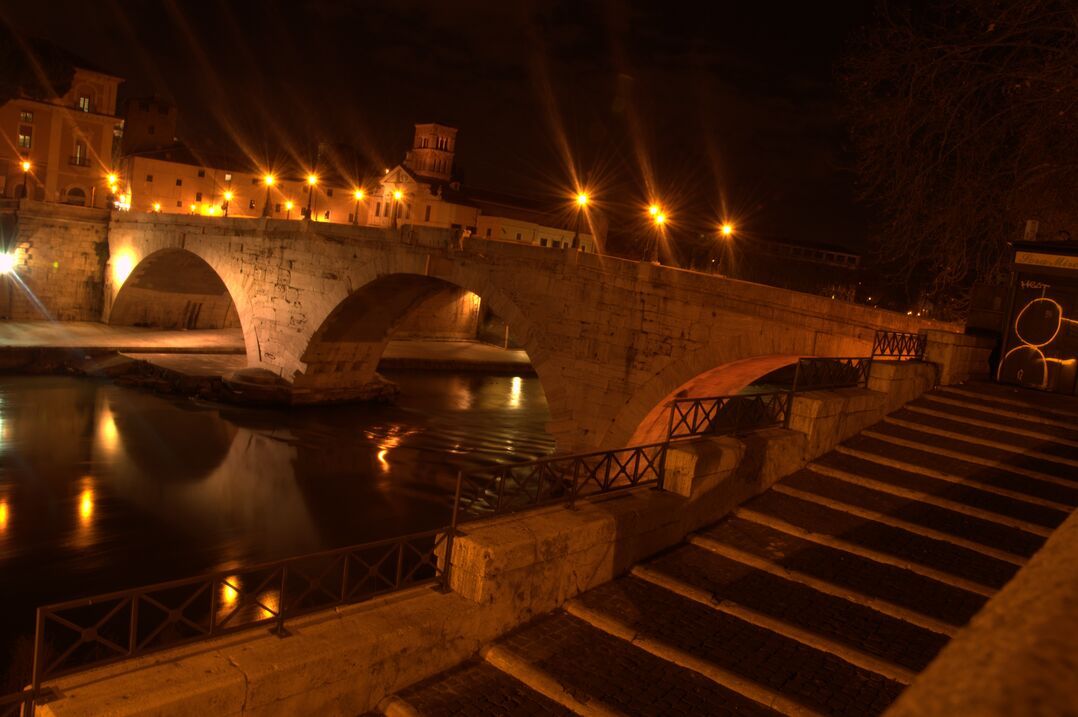
\includegraphics[width=\linewidth]{images/original/r0ea0825ft.jpeg}
    \caption{r0a966704t}
    \end{subfigure}\hfill%
    \begin{subfigure}[c]{.31\linewidth}\centering
    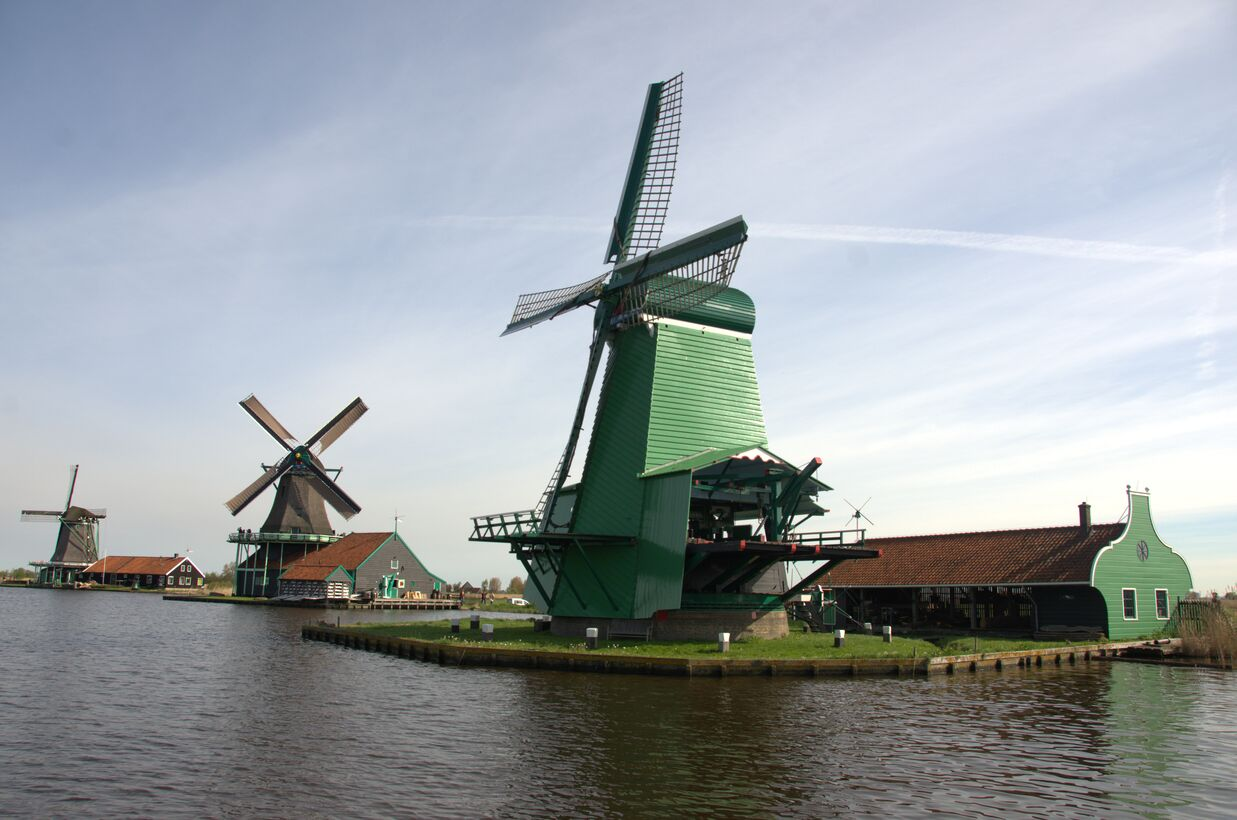
\includegraphics[width=\linewidth]{images/original/r1a0f5585t.jpeg}
    \caption{r0ea0825ft}
    \end{subfigure}
    
    \begin{subfigure}[c]{.31\linewidth}\centering
    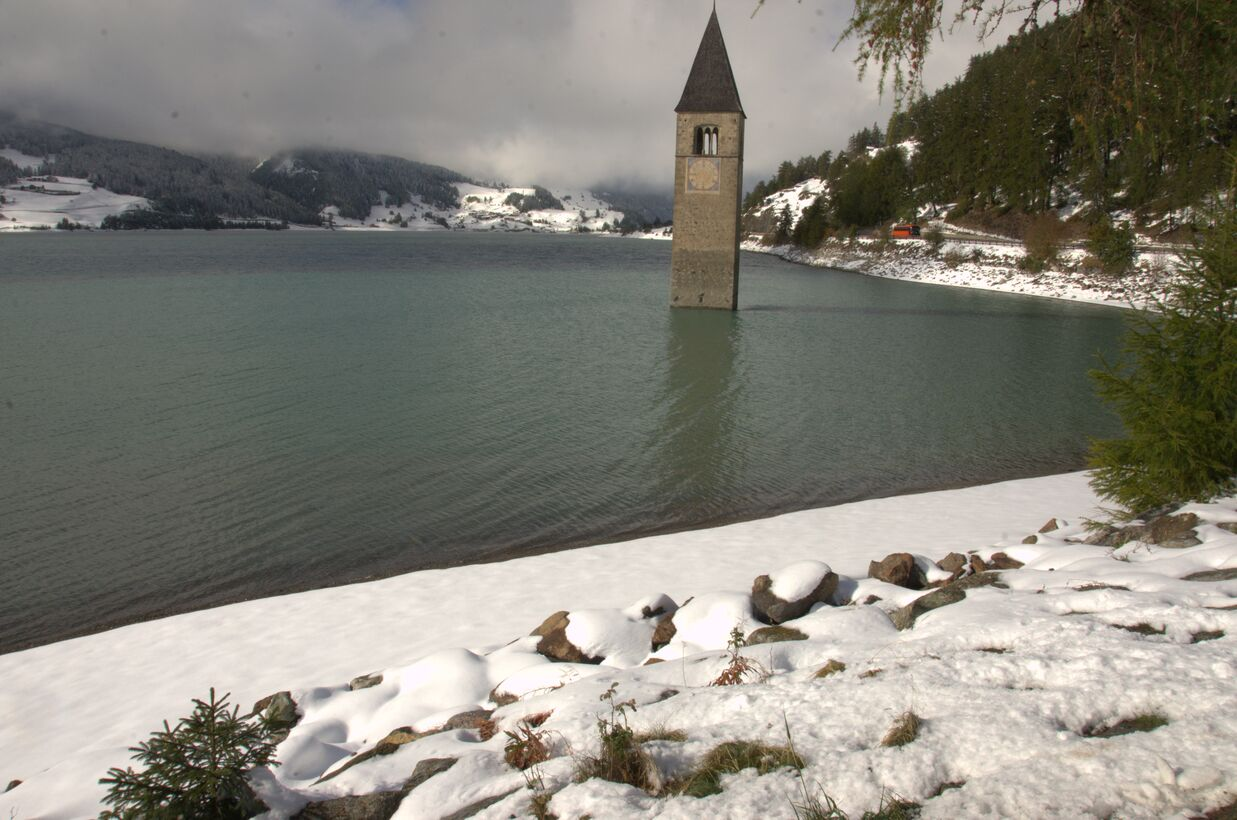
\includegraphics[width=\linewidth]{images/original/r1c9fdcf4t.jpeg}
    \caption{r0a2ff882t}
    \end{subfigure}\hfill%
    \begin{subfigure}[c]{.31\linewidth}\centering
    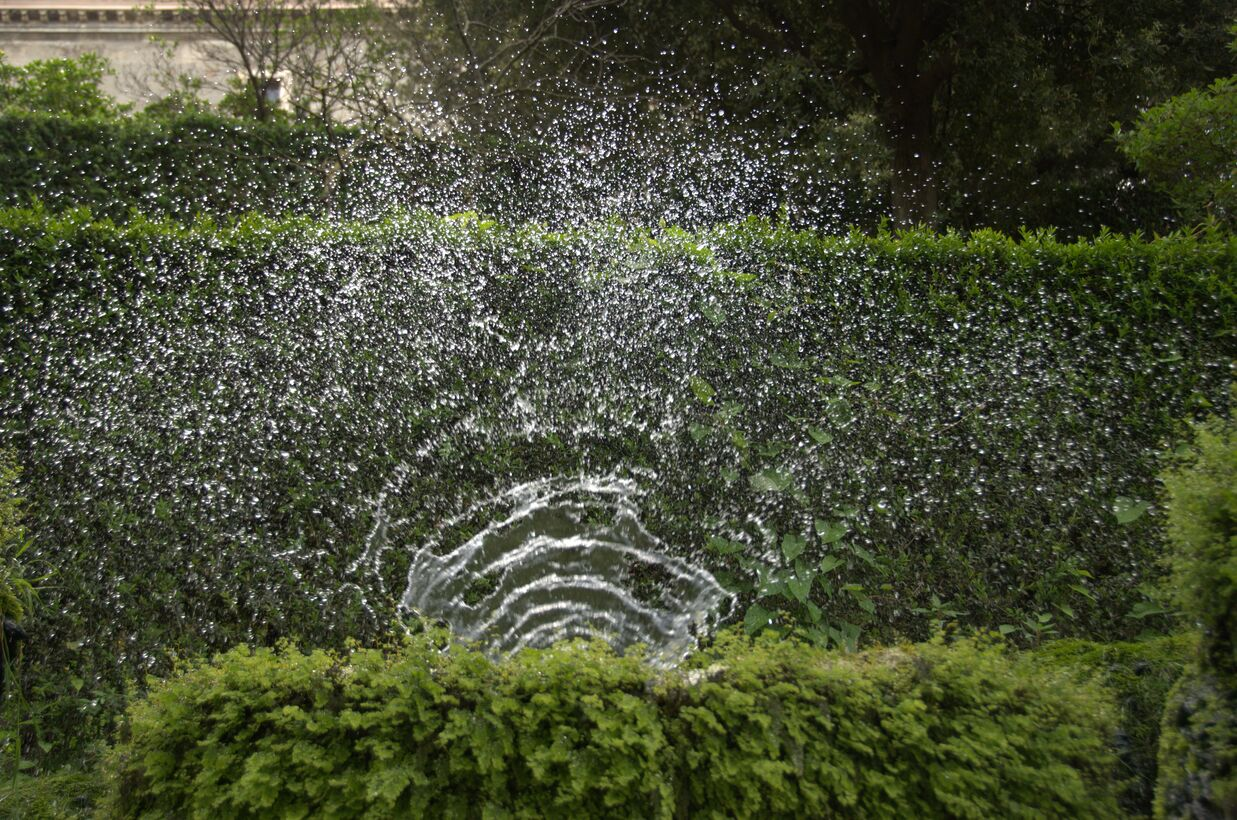
\includegraphics[width=\linewidth]{images/original/r06aa7dabt.jpeg}
    \caption{r0a966704t}
    \end{subfigure}\hfill%
    \begin{subfigure}[c]{.31\linewidth}\centering
    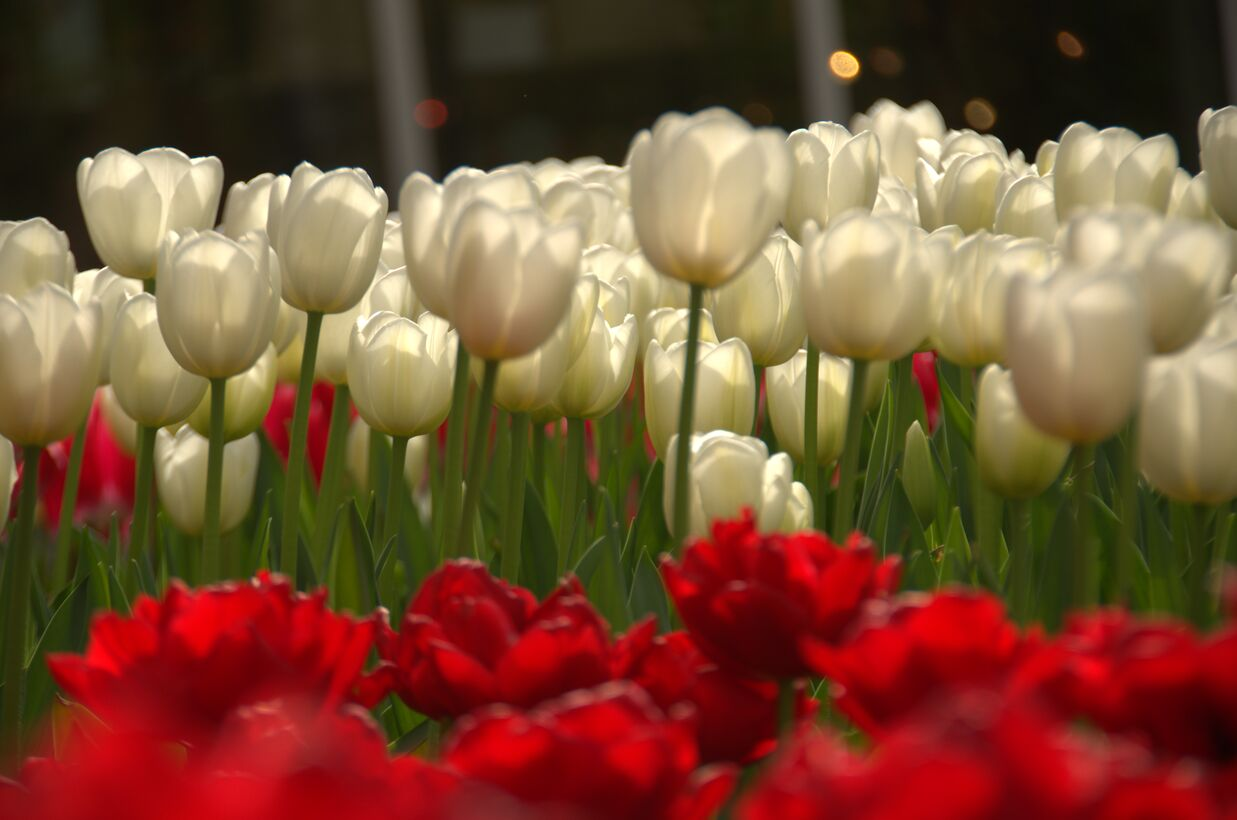
\includegraphics[width=\linewidth]{images/original/r07cfb432t.jpeg}
    \caption{r0ea0825ft}
    \end{subfigure}
    
    \begin{subfigure}[c]{.31\linewidth}\centering
    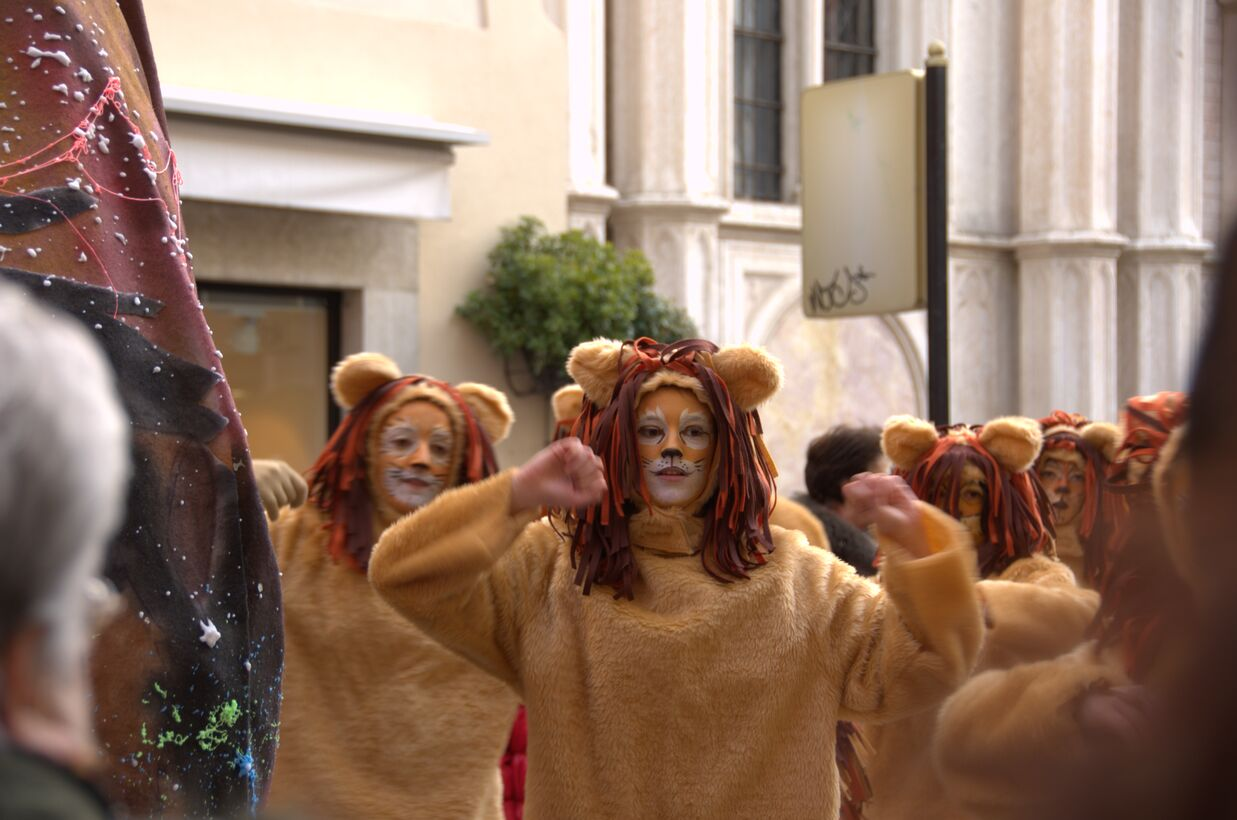
\includegraphics[width=\linewidth]{images/original/r07ffdc87t.jpeg}
    \caption{r0a2ff882t}
    \end{subfigure}\hfill%
    \begin{subfigure}[c]{.31\linewidth}\centering
    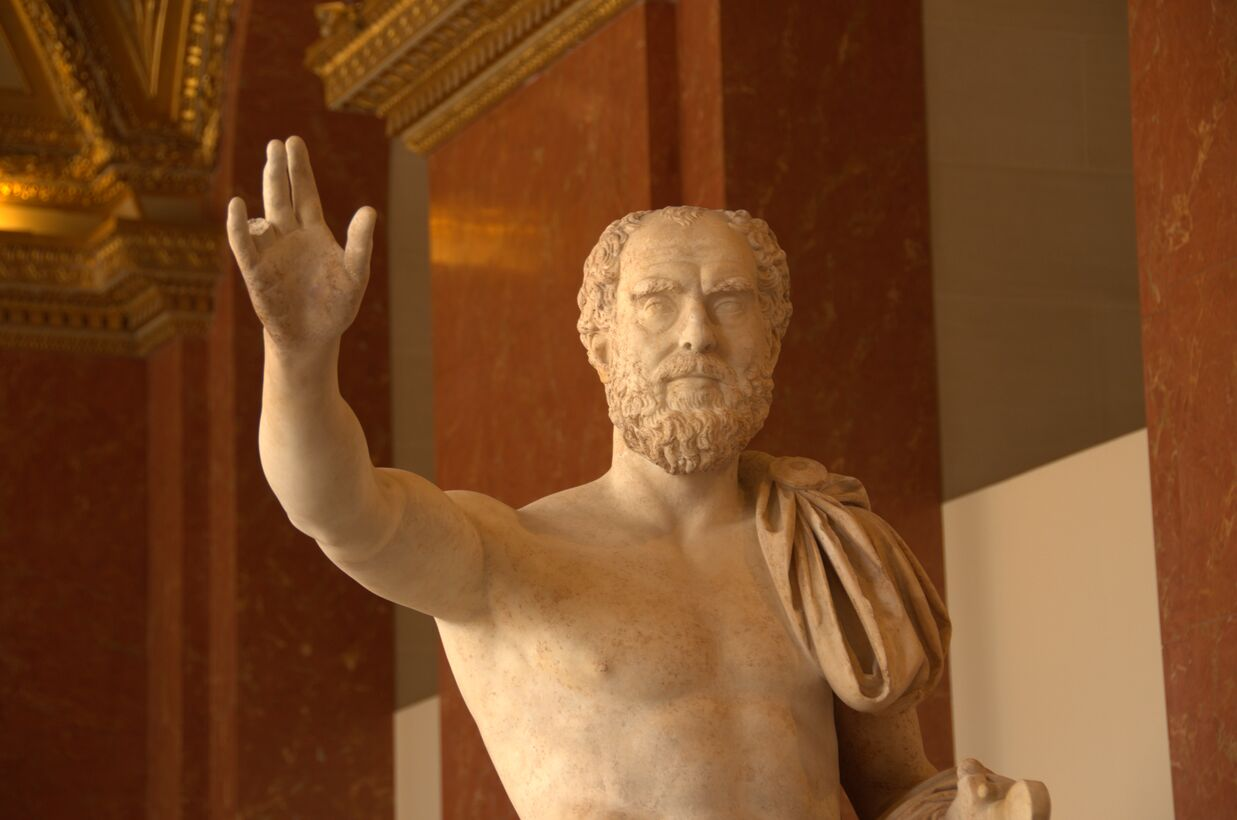
\includegraphics[width=\linewidth]{images/original/r16da5576t.jpeg}
    \caption{r0a966704t}
    \end{subfigure}\hfill%
    \begin{subfigure}[c]{.31\linewidth}\centering
    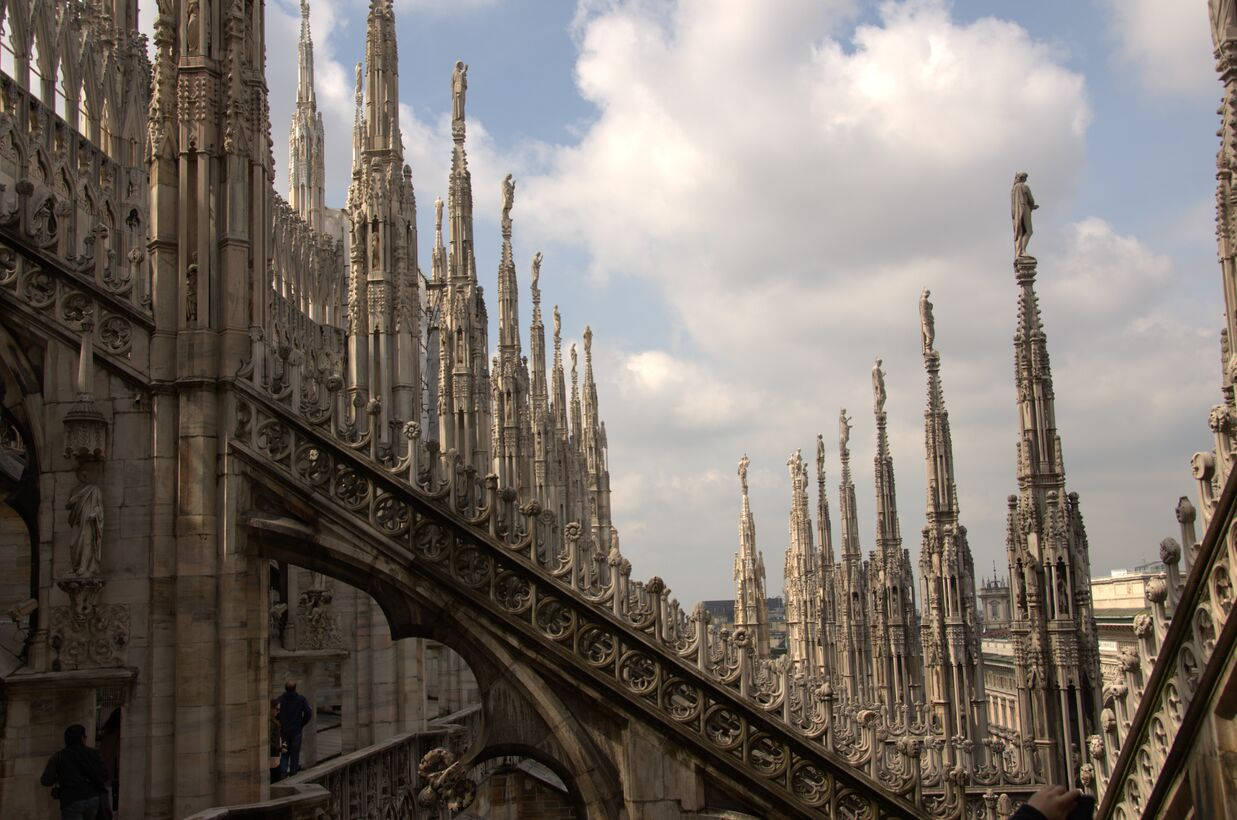
\includegraphics[width=\linewidth]{images/original/r191f3cdet.jpeg}
    \caption{r0ea0825ft}
    \end{subfigure}
    
    \caption{Those 15 images from the Raise Dataset~\cite{raise} were used during our experiments.}
    \label{fig:15images}
\end{figure}

\subsection{CFA pattern detection}

\begin{table}[ht]
    \centering
    \begin{tabular}{lcc}
    \toprule
    Demosaicking & Diagonal & Full pattern\\
    \midrule
    AAHD & \color{c2}0/15 & \color{c2}0/15\\
    AHD & \color{c0}15/15 & \color{c0}15/15\\
    DCB & \color{c0}15/15 & \color{c0}15/15\\
    DHT & \color{c2}3/15 & \color{c2}3/15\\
    Bilinear & \color{c0}15/15 & \color{c0}15/15\\
    PPG & \color{c0}15/15 & \color{c3}13/15\\
    VNG & \color{c0}15/15 & \color{c3}14/15\\
    \bottomrule
    \end{tabular}
    \caption{Identification of the main diagonal and of the full pattern on the 15 images. The algorithm works very well when the demosaicking is done with AHD, DCB or Bilinear demosaicking, with a few errors on the full pattern against PPG- or VNG-demosaicked images. It fails to detect even the diagonal on AAHD- and DHT-demosaicked images}
    \label{tab:global}
\end{table}

\begin{figure}[ht]
\centering
\begin{subfigure}[c]{.6\linewidth}
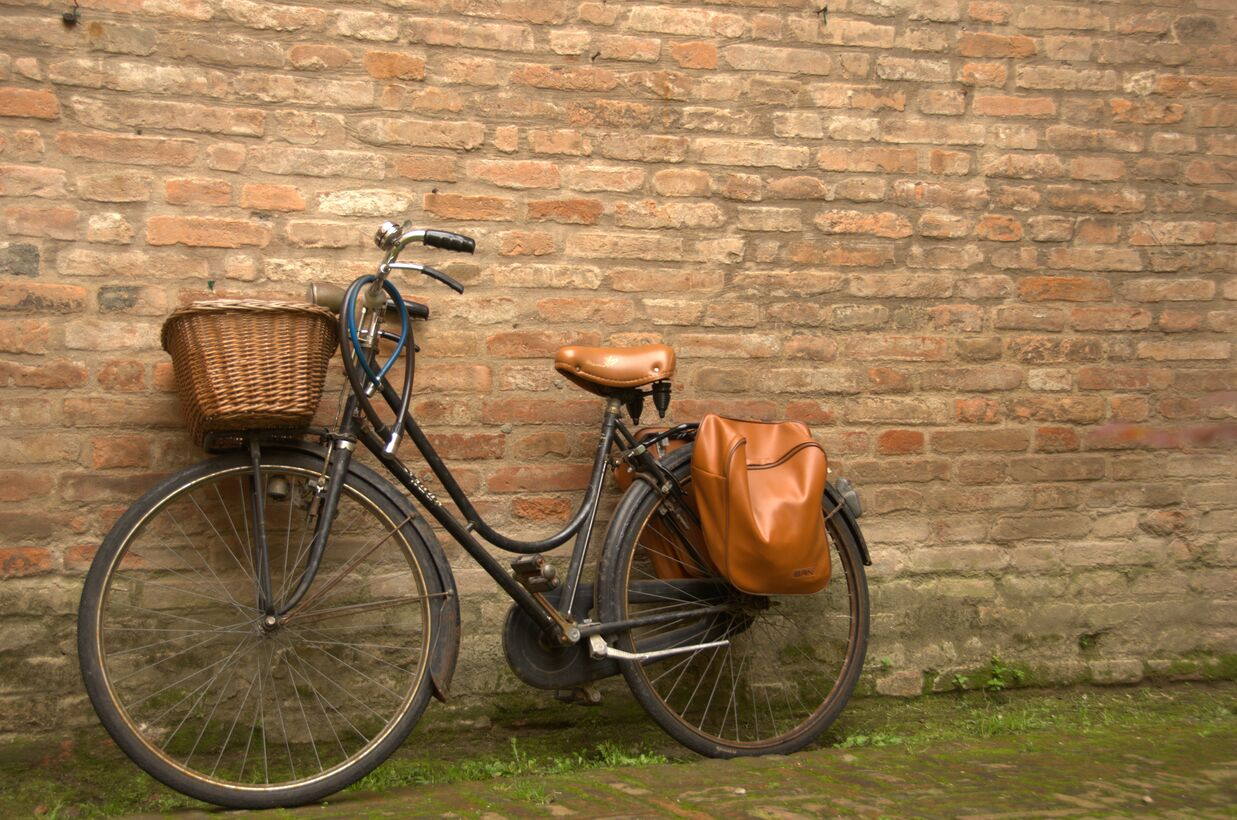
\includegraphics[width=\linewidth]{images/original/r0a2ff882t.jpeg}
\caption{original image (r0a2ff882t), in \textsc{rggb} pattern}
\end{subfigure}

\begin{subfigure}[c]{.14\linewidth}
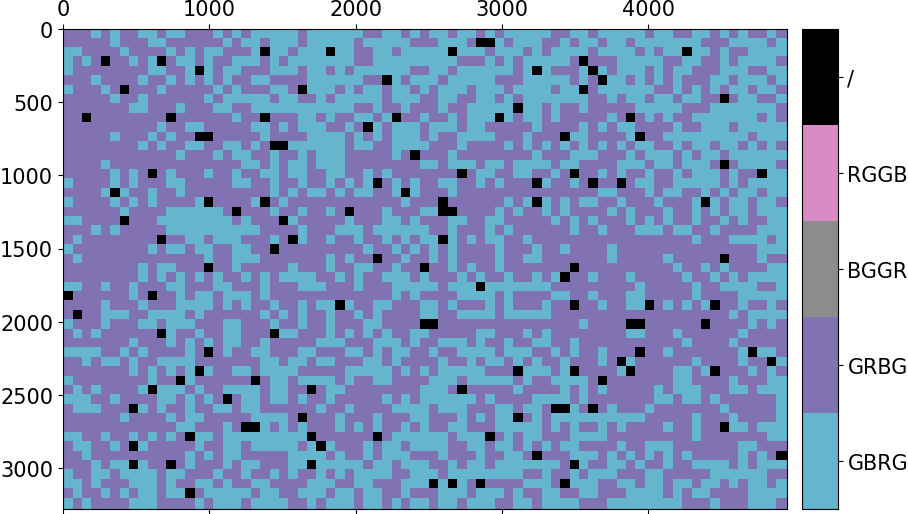
\includegraphics[width=\linewidth]{images/bike/AAHD/iso_64_grids.png}
\caption{AAHD, iso}
\end{subfigure}%
\begin{subfigure}[c]{.14\linewidth}
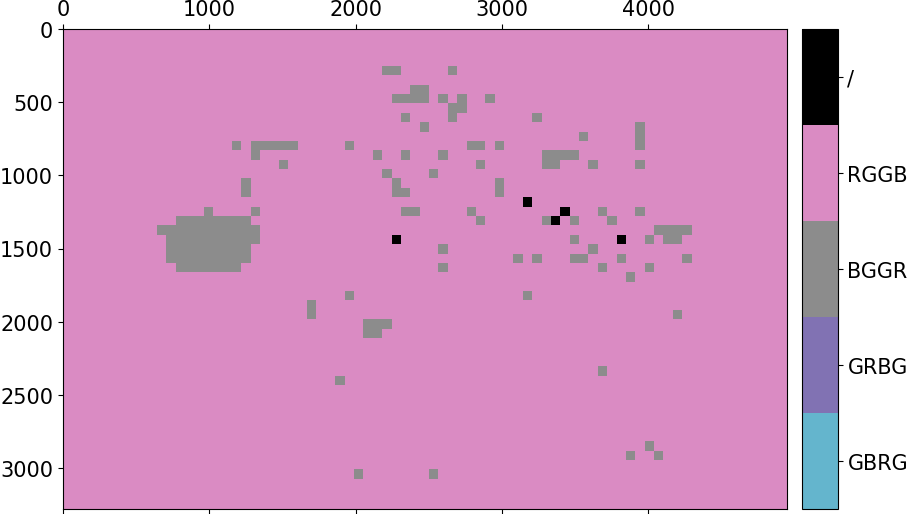
\includegraphics[width=\linewidth]{images/bike/AHD/iso_64_grids.png}
\caption{AHD, iso}
\end{subfigure}%
\begin{subfigure}[c]{.14\linewidth}

\includegraphics[width=\linewidth]{images/bike/DCB/iso_64_grids.png}
\caption{DCB, iso}
\end{subfigure}%
\begin{subfigure}[c]{.14\linewidth}
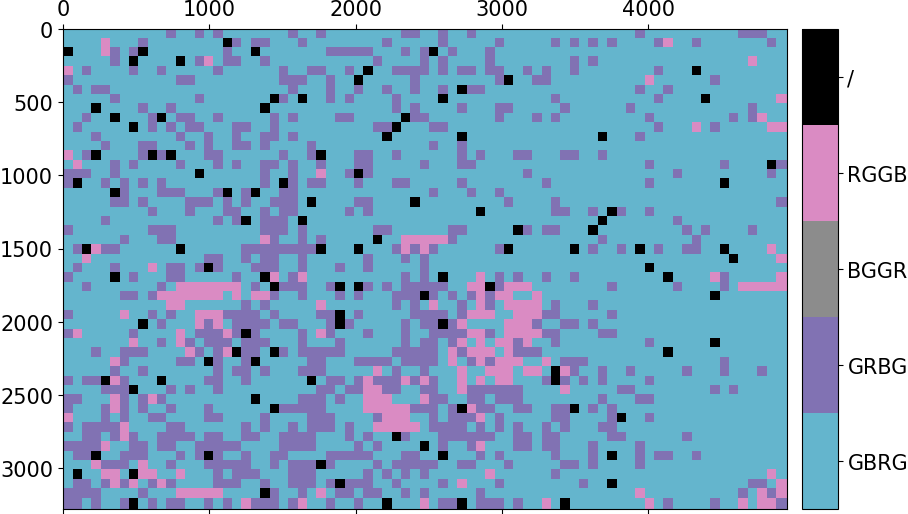
\includegraphics[width=\linewidth]{images/bike/DHT/iso_64_grids.png}
\caption{DHT, iso}
\end{subfigure}%
\begin{subfigure}[c]{.14\linewidth}

\includegraphics[width=\linewidth]{images/bike/LINEAR/iso_64_grids.png}
\caption{Bilinear, iso}
\end{subfigure}%
\begin{subfigure}[c]{.14\linewidth}
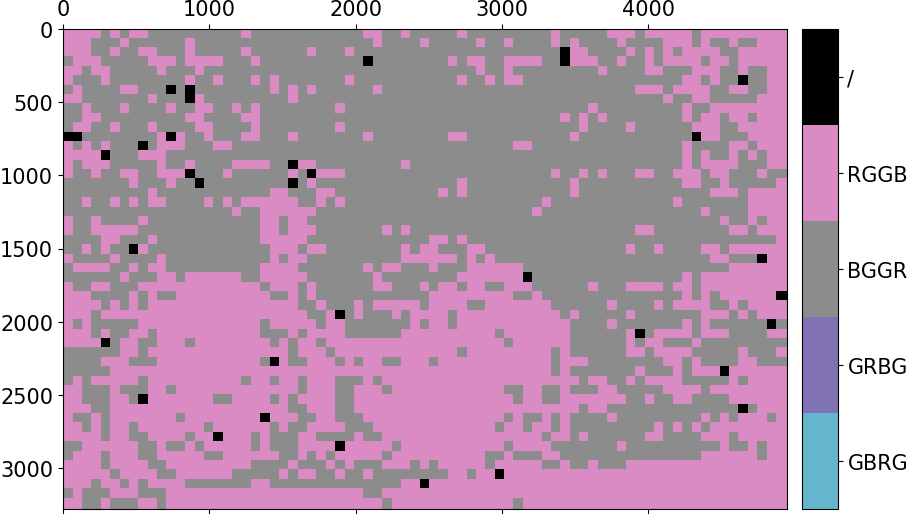
\includegraphics[width=\linewidth]{images/bike/PPG/iso_64_grids.png}
\caption{PPG, iso}
\end{subfigure}%
\begin{subfigure}[c]{.14\linewidth}
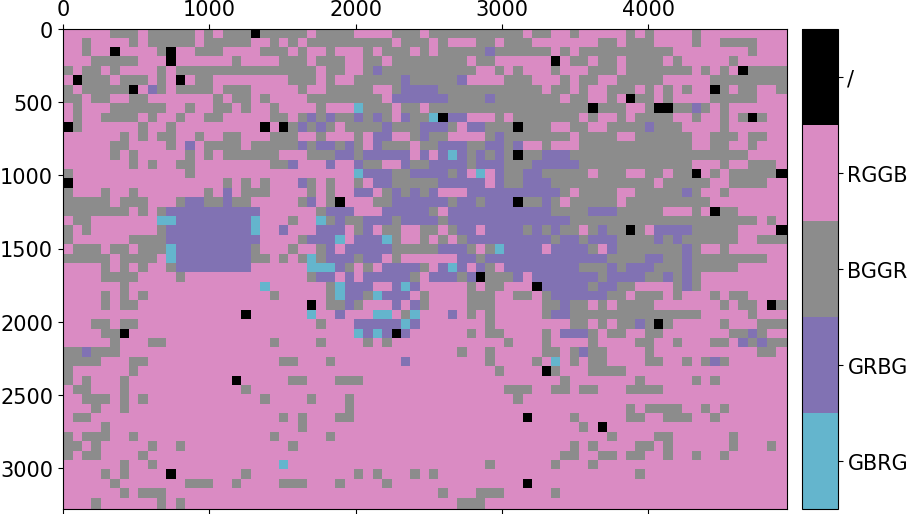
\includegraphics[width=\linewidth]{images/bike/VNG/iso_64_grids.png}
\caption{VNG, iso}
\end{subfigure}

\begin{subfigure}[c]{.14\linewidth}
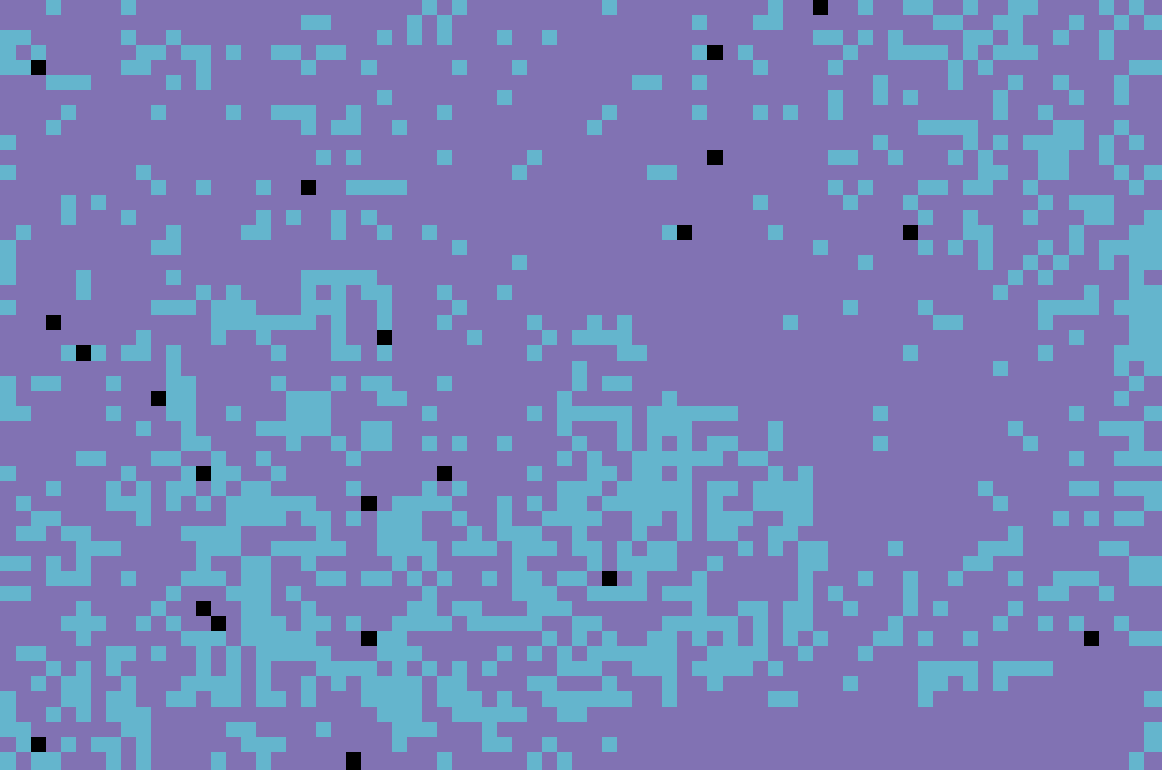
\includegraphics[width=\linewidth]{images/bike/AAHD/bid_64_grids.png}
\caption{AAHD, bi}
\end{subfigure}%
\begin{subfigure}[c]{.14\linewidth}
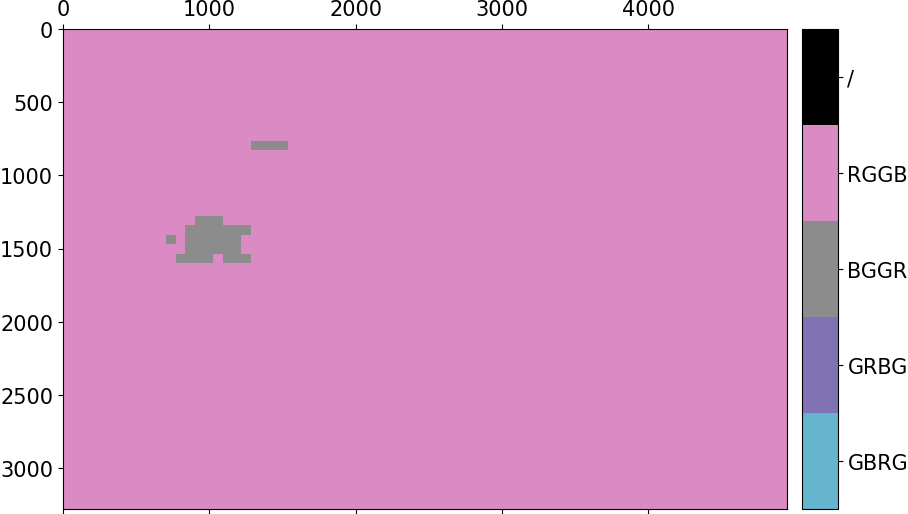
\includegraphics[width=\linewidth]{images/bike/AHD/bid_64_grids.png}
\caption{AHD, bi}
\end{subfigure}%
\begin{subfigure}[c]{.14\linewidth}
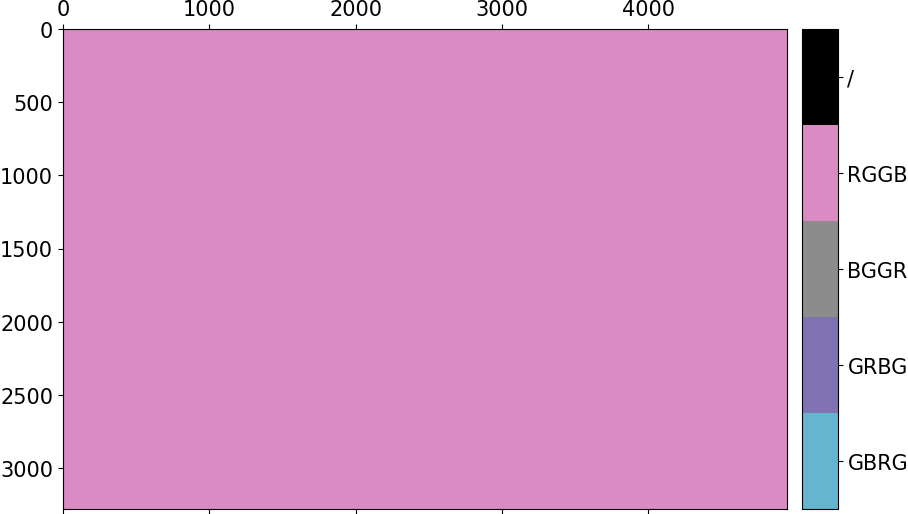
\includegraphics[width=\linewidth]{images/bike/DCB/bid_64_grids.png}
\caption{DCB, bi}
\end{subfigure}%
\begin{subfigure}[c]{.14\linewidth}
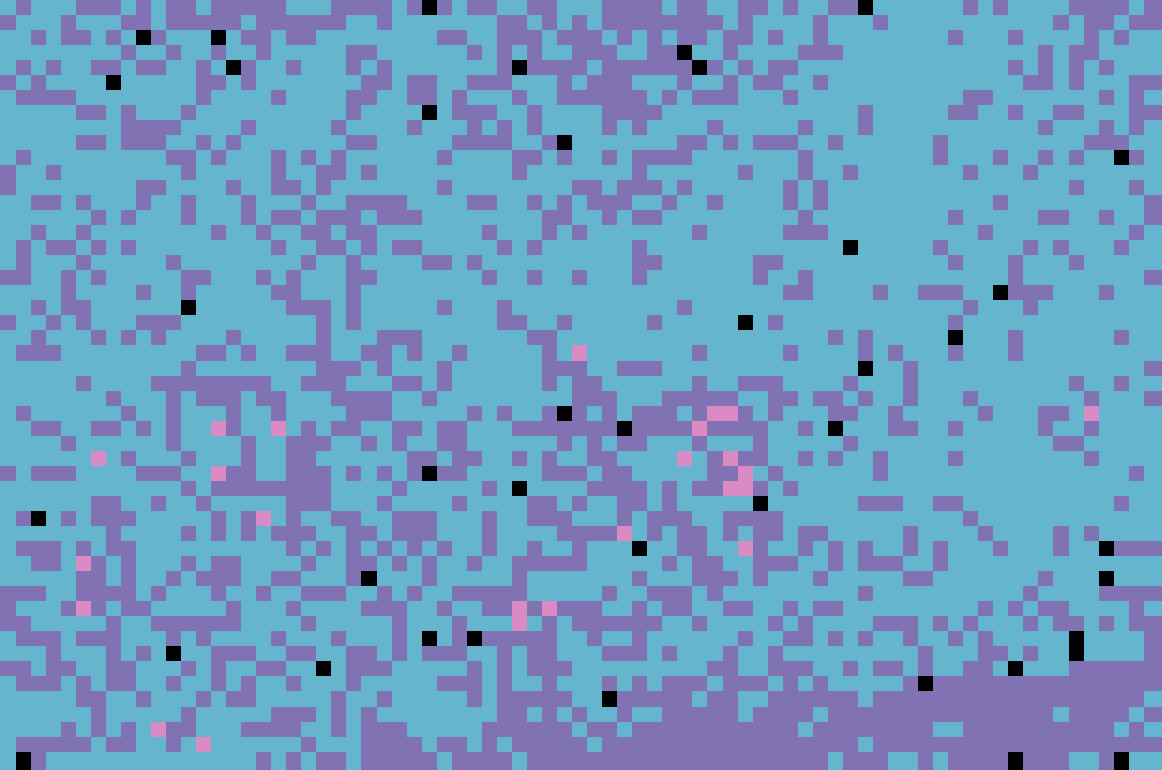
\includegraphics[width=\linewidth]{images/bike/DHT/bid_64_grids.png}
\caption{DHT, bi}
\end{subfigure}%
\begin{subfigure}[c]{.14\linewidth}

\includegraphics[width=\linewidth]{images/bike/LINEAR/bid_64_grids.png}
\caption{Bilinear, bi}
\end{subfigure}%
\begin{subfigure}[c]{.14\linewidth}
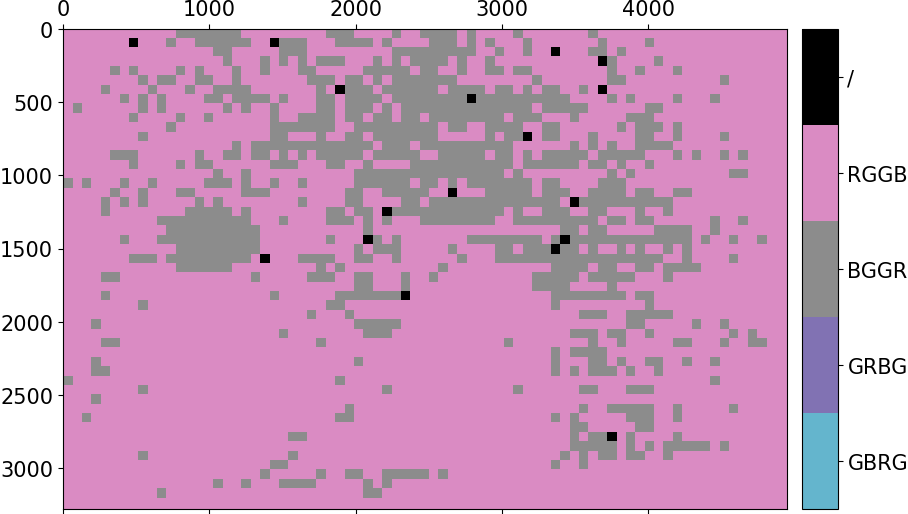
\includegraphics[width=\linewidth]{images/bike/PPG/bid_64_grids.png}
\caption{PPG, bi}
\end{subfigure}%
\begin{subfigure}[c]{.14\linewidth}
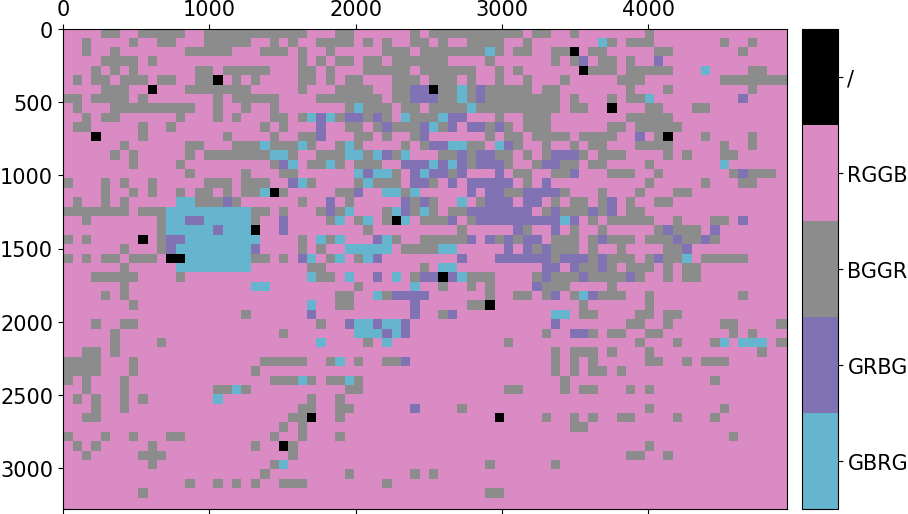
\includegraphics[width=\linewidth]{images/bike/VNG/bid_64_grids.png}
\caption{VNG, bi}
\end{subfigure}
\caption{Results of the method on 64×64 windows, both with the original isotropic intermediate value mask (iso) and the proposed bidirectional one (bi), on one image with the 7 different demosaicing algorithms. Both method work perfectly on the DCB- and Bilinear-demosaiced images. With the AHD, PPG and VNG methods, both methods have trouble discerning between the two patterns sharing the same diagonal, but the bidirectional detection makes fewer mistakes. Textured regions such as the basket can create a localized shift in the detected mosaic, which could be interpretated as a forgery.
With the AAHD and DHT algorithm, the method consistently detects the wrong diagonal.}
\label{fig:bike}
\end{figure}

\begin{figure}[ht]
\centering
\begin{subfigure}[t]{.5\linewidth}
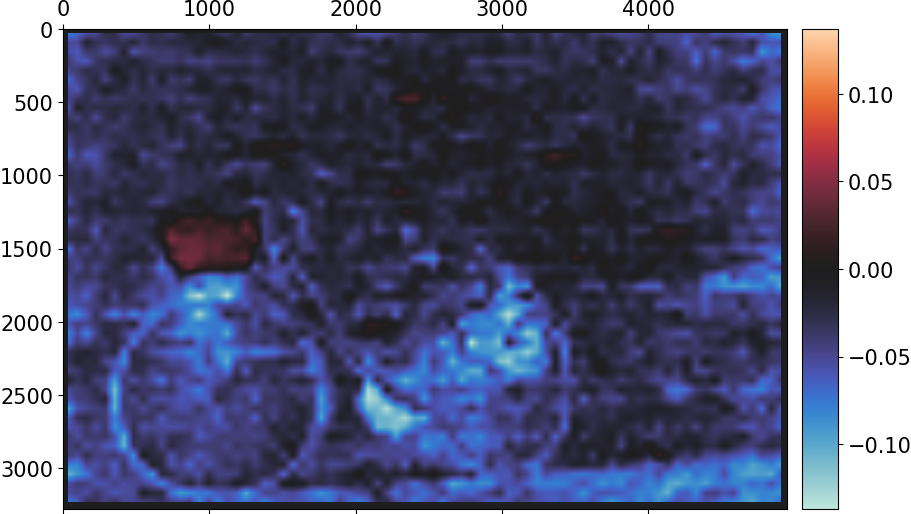
\includegraphics[width=\linewidth]{images/bike/ahd_iso_64_diff_rggb_bggr.png}
\caption{Isotropic}
\end{subfigure}%
\begin{subfigure}[t]{.5\linewidth}
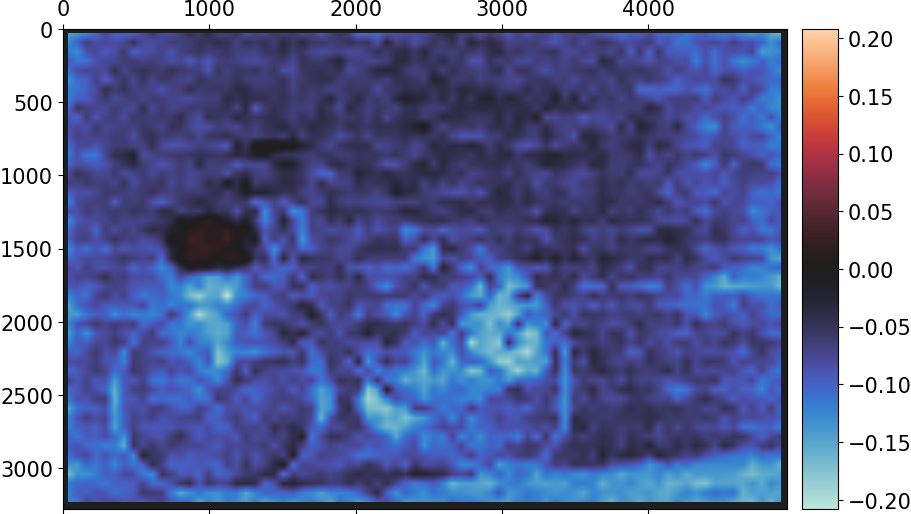
\includegraphics[width=\linewidth]{images/bike/ahd_bid_64_diff_rggb_bggr.png}
\caption{Bidirectional}
\end{subfigure}%
\caption{This figure shows, on the AHD-demosaiced bicycle image, the difference of counts of intermediate values corresponding to the \textsc{rggb} and \textsc{bggr} patterns, on the red and blue channels. This count is what is used by the algorithm to decide on a grid. A negative difference corresponds to the correct \textsc{rggb} pattern, a positive difference to the incorrect \textsc{bggr} pattern. The difference is normalized by dividing it by the size of the block ($64\times64$). The textures in the basket area leads to a locally consistent shift in the position of the intermediate values. The error is slightly less prominent when a bidirectional mask is used, but is still consistently in favour of the wrong grid.}
\end{figure}



\begin{itemize}
    \item On our database: global results, \% mask size, \% alg used, \% dual
    \item On the 15 images:
    \begin{itemize}
        \item Full image
        \item Results on windows
        \item JPEG
        \item Noise
        \item Median
    \end{itemize}
\end{itemize}
%------------------------------------------------------------------------------
\section{Limitations}

%------------------------------------------------------------------------------
\section{Conclusion}

Here is the conclusion

%------------------------------------------------------------------------------
\section*{Acknowledgment}


%------------------------------------------------------------------------------
\section*{Image Credits}
{\small\flushleft

}

%------------------------------------------------------------------------------
\bibliographystyle{siam}
\bibliography{article}

\end{document}
%------------------------------------------------------------------------------